\documentclass{article}

% formato
\usepackage[margin = 1.5cm, letterpaper]{geometry}
\usepackage[utf8]{inputenc}

% autómatas
\usepackage{tikz}
\usetikzlibrary{automata, positioning}

%formato ecuaciones
\usepackage{amsmath}

% símbolos
\usepackage{amssymb}

% manejo de tablas
\usepackage{float}

\begin{document}
    \title{
        Autómatas y Lenguajes formales \\
        Ejercicio Semanal 5
    }

    \author{
        Sandra del Mar Soto Corderi \\
        Edgar Quiroz Castañeda
    }

    \date{
        7 de marzo del 2019
    }
    
    \maketitle

    \begin{enumerate}
        \item {
            Para cada lenguaje responda los incisos
            \begin{enumerate}
                \item Diseña un AFN (sin $\epsilon-transiciones$) que acepte a 
                $L$
                \item Muestra el procesamiento formal de las cadenas $aabbbb$ y 
                $abaab$ usando la función $\delta^{*}$.
                \item Transforma M a un AFD mediante la construcción de 
                subconjuntos.
            \end{enumerate}
            \begin{itemize}
                \item $L = (a + b)^{*}(aaa + bbb)(a + b)^{*}$
                \begin{enumerate}
                    \item {
                        El autómata sería
                        \begin{align*}
                            M &= \langle Q, \Sigma, \delta, q_{0}, F \rangle \ con\\
                            Q &= \{q_{0}, q_{1}, q_{2}, q_{3}, q_{4}, q_{5}\} \\
                            \Sigma &= \{a, b\} \\
                            q_{0} &= q_{0} \\
                            F &= \{q_{5}\}
                        \end{align*}
                        Y con función de transición $\delta$
                        
                        \begin{table}[H]
                            \centering
                            \begin{tabular}{|c|c|c|c|c|c|c|}
                                \hline
                                $\delta$ & $q_{0}$ & $q_{1}$ & $q_{2}$ & $q_{3}$ 
                                & $q_{4}$ & $q_{5}$\\
                                \hline
                                $a$ & $\{q_{0}, q_{1}\}$ & $\{q_{2}\}$ & $\{q_{5}\}$ 
                                & $\varnothing$ & $\varnothing$ & $\{q_{5}\}$ \\
                                \hline
                                $b$ & $\{q_{0}, q_{3}\}$ & $\varnothing$ 
                                & $\varnothing$ & $\{q_{4}\}$ & $\{q_{5}\}$ 
                                & $\{q_{5}\}$ \\
                                \hline
                            \end{tabular}
                        \end{table}

                        Con representación gráfica.
                        \begin{center}
                            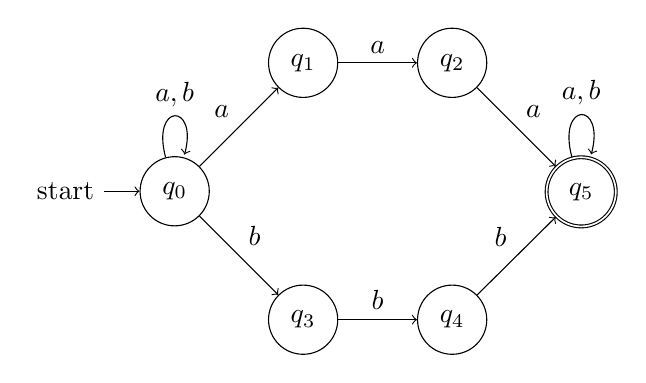
\begin{tikzpicture}[auto]
                                % estados
                                \node [state, initial] (q0) {$q_{0}$};
                                \node [state] (q1) [above right=of q0] {$q_{1}$};
                                \node [state] (q2) [right=of q1] {$q_{2}$};
                                \node [state] (q3) [below right=of q0] {$q_{3}$};
                                \node [state] (q4) [right=of q3] {$q_{4}$};
                                \node [state, accepting] (q5) [below right=of q2] {$q_{5}$};
    
                                % transiciones
                                \path[->]
                                (q0) edge [loop above] node {$a, b$} (q0)
                                     edge node {$a$} (q1)
                                     edge node {$b$} (q3)
                                (q1) edge node {$a$} (q2)
                                (q2) edge node {$a$} (q5)
                                (q3) edge node {$b$} (q4)
                                (q4) edge node {$b$} (q5)
                                (q5) edge [loop above] node {$a, b$} (q5);
                            \end{tikzpicture}
                        \end{center}
                    }
                \end{enumerate}
                
                    
                

                \item $L = \{a^{n} b^{m} | n + m \ es\ par \}$
                \begin{enumerate}
                	\item {
                		El autómata sería
                		\begin{align*}
                		M &= \langle Q, \Sigma, \delta, q_{0}, F \rangle \ con\\
                		Q &= \{q_{0}, q_{1}\} \\
                		\Sigma &= \{a, b\} \\
                		q_{0} &= q_{0} \\
                		F &= \{q_{0}\}
                		\end{align*}
                		Y con función de transición $\delta$
                		
                		\begin{table}[H]
                			\centering
                			\begin{tabular}{|c|c|c|}
                				\hline
                				$\delta$ & $q_{0}$ & $q_{1}$ \\
                				\hline
                				$a$ & $\{q_{0}\}$ & $\{q_{1}\}$ \\
                				\hline
                				$b$ & $\{q_{1}\}$ & $\{q_{0}\}$ \\
                				\hline
                			\end{tabular}
                		\end{table}
                		
                		Con representación gráfica.
                		\begin{center}
                			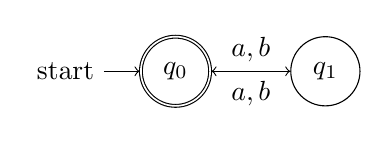
\begin{tikzpicture}[auto]
                			% estados
                			\node [state, accepting, initial] (q0) {$q_{0}$};
                			\node [state] (q1) [right=of q0] {$q_{1}$};
                			                			
                			% transiciones
                			\path[->]
                			(q0)edge node {$a, b$} (q1)
                			(q1)edge node {$a, b$} (q0);
                			\end{tikzpicture}
                		\end{center}
                	}
                \end{enumerate}
            \end{itemize}
            
        }
    \end{enumerate}
\end{document}